\chapter{Experiments}
In this chapter, BVBMC is applied in a number of examples, as to show the algorithm behavior in different scenarios. The examples consists of estimating continuous probability densities in up to $10$ dimensions \footnote{In more than $10$ dimensions, performance was very poor. What was seen is that the algorithm got \enquote{stuck} in its first component proposal, and could not find new components to be proposed with acceptable weights.}.

\section{1-d Mixture of Gaussians}

As a showcase example, a one-dimensional mixture of Gaussians is considered
\begin{displaymath}
 f(x) = \sum_{i=1}^{12} w_i \mathcal{N}(x;\mu_i,\sigma^2_i),
\end{displaymath}
with $w_i = \frac{1}{12}$, $\mu_i \sim \mathcal{N}(0,\sqrt{5})$ and $\sigma^2_i = 1$. This results in a many-peaked distribution, with mean $\mu_0=-1.6585$ and variance $\sigma^2_0 = 25.0316$, whose density is shown in Figure \ref{target1dmixture}. 

In each example, the quality of the approximation by the BVBMC algorithm is measured, by calculating both the difference between the estimated mean $\mu$ and the true mean $\mu_0$, in $\log_{10}|\mu - \mu_0|$, and the difference between the estimated variance $\sigma^2$ and the true variance $\sigma^2_0$, in $\log_{10}(|\sigma^2-\sigma^2_0|/|\sigma^2_0|)$. Code for this section can be found in \url{https://github.com/DFNaiff/Dissertation/tree/master/tests_dissertation/illustrative}. 

\begin{figure}
	\centering
	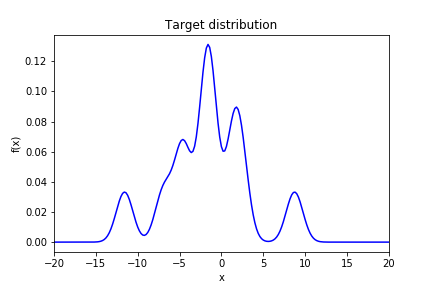
\includegraphics[width=0.7\linewidth]{figs/targetexil1a.png}
	\caption{\label{target1dmixture} Target distribution.}
\end{figure}

\subsection{Passive evaluation}
In the first two examples, the target evaluations of $\log f(x)$ were done in a uniform grid from $-20$ to $20$ with $51$ points, resulting in the GP replicating almost exactly the target distribution. This is done to illustrate the algorithm's capacity to generate good approximate distributions, if the GP approximates closely the (unnormalized) target distribution. Output scaling was done by normalizing, as discussed in Section \ref{outputscaling}. The GP mean was chosen to be constant, setting it with the heuristic corresponding to the \textit{normalize} scaling, as discussed in Section \ref{meansection}.

\subsubsection{Influence of kernel in approximation}
It was tested the kernel influence on the final approximation. For this, the tested kernels were $k_{\text{PMat},1/2}$, $k_{\text{PMat},2/2}$, $k_{\text{PMat},5/2}$ and $k_{\text{SQE}}$. The algorithm was run for 50 iterations, with joint parameter updating done every 10 steps. The results are shown in Figure \ref{kernelcomparison}.

There is an interesting behavior to be seen, in that the GP approximation for the kernels $k_{\text{PMat},1/2}$ and  $k_{\text{PMat},3/2}$ were considerably more accurate than with kernels $k_{\text{PMat},5/2}$ and $k_{\text{SQE}}$. However, this accuracy in the GP approximation does not reflect in a better posterior approximation, that are seen with $k_{\text{PMat},5/2}$ and $k_{\text{SQE}}$. This may be due to the fact that the first two kernels makes for GP approximations that are too rough, making it difficult to be approximated by the BVBMC algorithm.

\begin{figure}
	\centering
	\subfloat[$k_{\text{PMat},1/2}$, moments.]{\label{fig11a}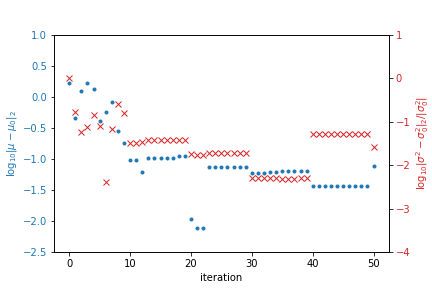
\includegraphics[width=0.4\linewidth]
		{figs/dmcil1fk12.png}}
	\subfloat[$k_{\text{PMat},1/2}$, final result.]{\label{fig11b}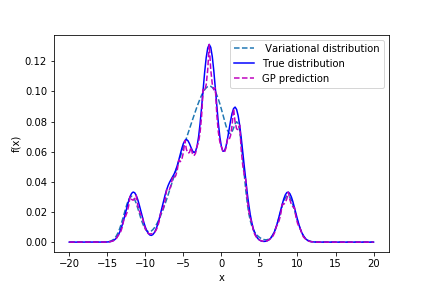
\includegraphics[width=0.4\linewidth]
	{figs/convgraphil1fk12.png}}

	\subfloat[$k_{\text{PMat},3/2}$, moments.]{\label{fig11a}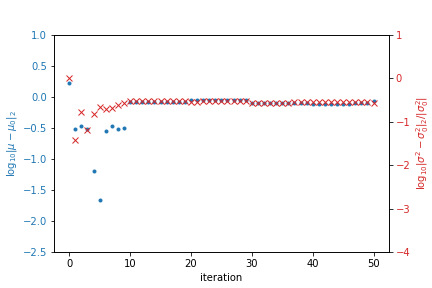
\includegraphics[width=0.4\linewidth]
	{figs/dmcil1fk32.png}}
\subfloat[$k_{\text{PMat},3/2}$, final result.]{\label{fig11b}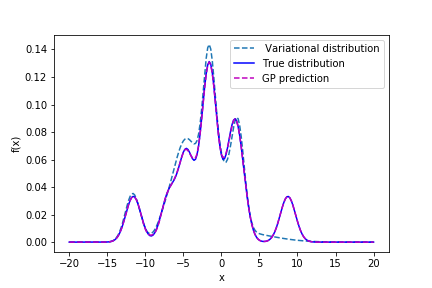
\includegraphics[width=0.4\linewidth]
	{figs/convgraphil1fk32.png}}

	\subfloat[$k_{\text{PMat},5/2}$, moments.]{\label{fig11a}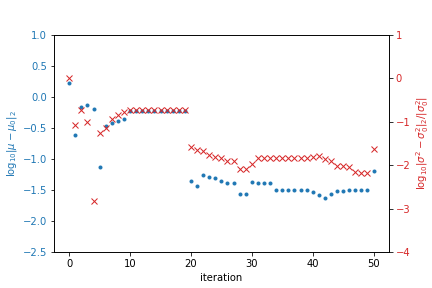
\includegraphics[width=0.4\linewidth]
	{figs/dmcil1fk52.png}}
\subfloat[$k_{\text{PMat},5/2}$, final result.]{\label{fig11b}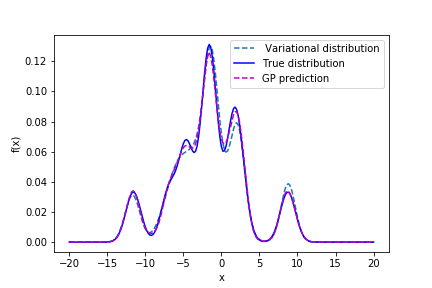
\includegraphics[width=0.4\linewidth]
	{figs/convgraphil1fk52.png}}

	\subfloat[$k_{\text{SQE}}$, moments.]{\label{fig11a}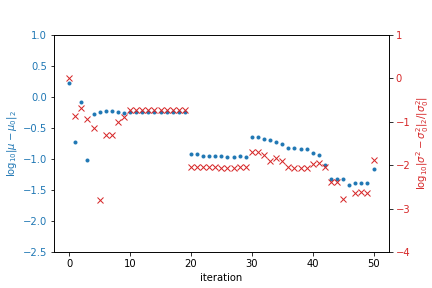
\includegraphics[width=0.4\linewidth]
	{figs/dmcil1fkSQE.png}}
\subfloat[$k_{\text{SQE}}$, final result.]{\label{fig11b}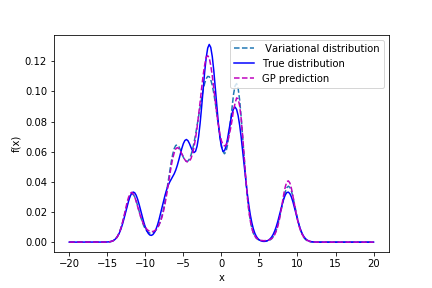
\includegraphics[width=0.4\linewidth]
	{figs/convgraphil1fkSQE.png}}
	\caption[Accuracy analysis for different kernels.]{\label{kernelcomparison} Accuracy analysis for different kernels. Each row corresponding to one kernel, in order being $k_{\text{PMat},1/2}$, $k_{\text{PMat},2/2}$, $k_{\text{PMat},5/2}$ and $k_{\text{SQE}}$. The first column (MC) shows the accuracy of mean (blue), and variance (red), while the second column shows the the predicted density, the true density and the GP approximation of the density.}
\end{figure}

\subsubsection{Influence of training routine in approximation}
Next, it was tested the difference that the training routine makes on both accuracy and algorithm running time. For this, using the same setting as above with kernel $k_{\text{PMat},5/2}$, three training routines were tested:
\begin{itemize}
	\item Running the algorithm for 50 iterations, with joint parameter updating done every step (training routine A).
	\item Running the boosting algorithm for 50 iterations, with joint parameter updating done every 10 steps (training routine B).
	\item Running the boosting algorithm for 50 iterations, with no joint parameter updating (training routine C).
\end{itemize}

The results are shown in Figure \ref{trainingcomparison}.  It can be seen that training routine B performs considerably better than routine A and routine C, while training routine A and training routine B has comparable final performance, with routine A converging in fewer iterations. As of running time, it can be see that for training routine A it increases quadratically in relation to the number of iterations, while for training routine C it increases linearly. As for training routine B, the running time increases linearly except to jumps corresponding to joint parameter updating, with each jump size growing with the iteration.

It is interesting to pause and consider the behavior of training routine B, since in the next set of examples this were the routine used, with some differences of number of iterations and intervals between joint parameter updating. Notice that boosting improves considerably accuracy up to the first joint parameter updating, in 10 iterations, and after this many intervals between two joint parameter updating essentially shows no improvements. This suggests that a smarter training routine, involving boosting only in the initial steps may be desirable. This idea was not explored further in this dissertation.

\begin{figure}
	\centering
	\subfloat[Routine A, moments]{\label{fig11a}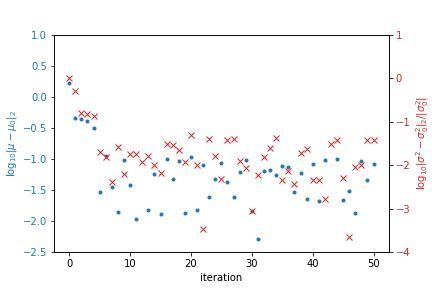
\includegraphics[width=0.35\linewidth]
		{figs/dmcil1ati1.png}}
	\subfloat[Routine A, final result.]{\label{fig11b}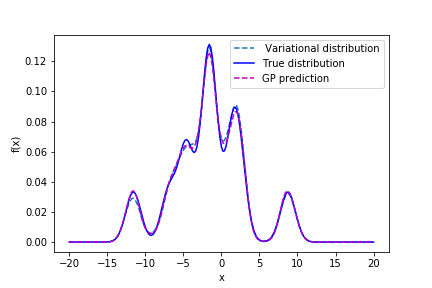
\includegraphics[width=0.35\linewidth]
		{figs/convgraphil1ati1.png}}
	\subfloat[Routine A, running time.]{\label{fig11b}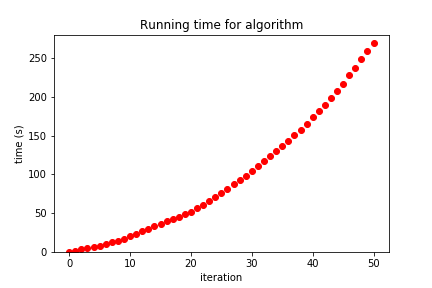
\includegraphics[width=0.35\linewidth]
	{figs/timegraphil1ati1.png}}

	\subfloat[Routine B,moments.]{\label{fig11a}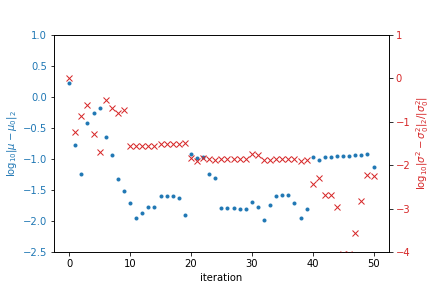
\includegraphics[width=0.35\linewidth]
		{figs/dmcil1ati10.png}}
	\subfloat[Routine B, final result.]{\label{fig11b}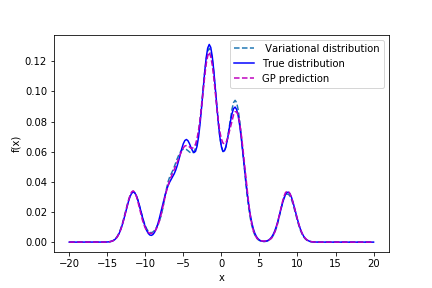
\includegraphics[width=0.35\linewidth]
		{figs/convgraphil1ati10.png}}
	\subfloat[Routine B, running time.]{\label{fig11b}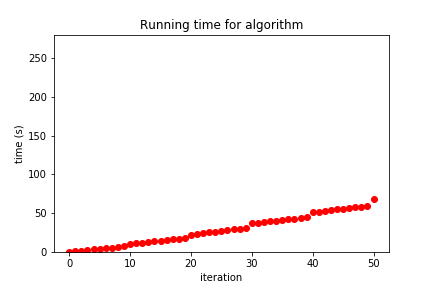
\includegraphics[width=0.35\linewidth]
	{figs/timegraphil1ati10.png}}

	\subfloat[Routine C, moments.]{\label{fig11a}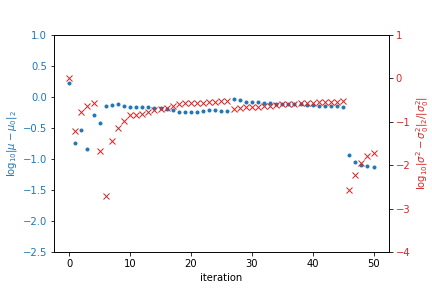
\includegraphics[width=0.35\linewidth]
		{figs/dmcil1ati1000.png}}
	\subfloat[Routine C, final result.]{\label{fig11b}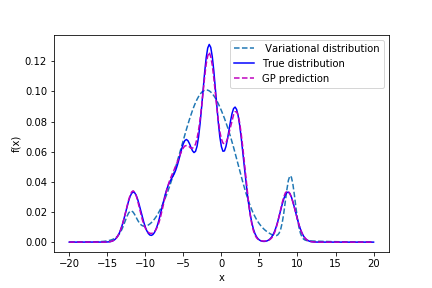
\includegraphics[width=0.35\linewidth]
		{figs/convgraphil1ati1000.png}}
	\subfloat[Routine C, running time.]{\label{fig11b}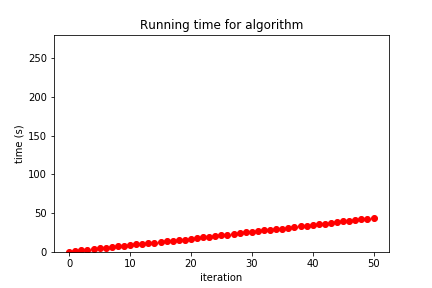
\includegraphics[width=0.35\linewidth]
	{figs/timegraphil1ati1000.png}}

	\caption[Accuracy analysis for different training routines.]{\label{trainingcomparison} Accuracy analysis for different training routines. Each row corresponding to training routine A, B and C, respectively. The first column shows the accuracy of mean (blue) and (red), the second column show the difference between the predicted density, the true density and the GP approximation of the density, and the third column shows the algorithm running time at each step.}
\end{figure}

\subsection{Active evaluation}
In this example, it is considered how BVBMC performs with active evaluation. For all examples, $5$ initial evaluation points are sampled randomly, with distribution $\mathcal{N}(0,\sqrt{10})$. Subsequently, at each iteration an evaluation point is chosen according to the running acquisition function. Four acquisition functions were tested: uncertainty sampling (US, \eqref{us_vbmc}), prospective prediction (PROP, \eqref{prospective_vbmc}), moment-matched log transform (MMLT, \eqref{mmlt_vbmc}), and prospective moment-matched log transform (MMLT$_P$, \eqref{mmltprop_vbmc}). The results are shown in Figure \ref{acquisition}. There it can be seen that all acquisition function performed well, although the GP approximation is better for the PROP and MMLT acquisitions.

\begin{figure}
	\centering
	\subfloat[US, moments.]{\label{fig11a}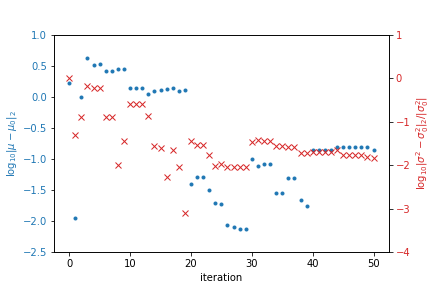
\includegraphics[width=0.35\linewidth]
		{figs/dmcil1g_aq_uncertainty_sampling.png}}
	\subfloat[US, final result.]{\label{fig11b}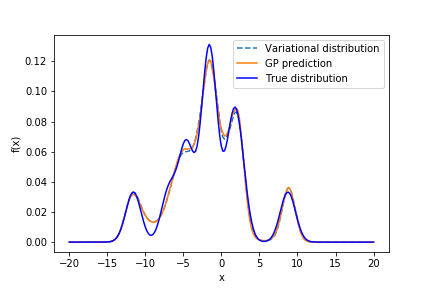
\includegraphics[width=0.35\linewidth]
		{figs/convgraphil1g_aq_uncertainty_sampling.png}}
	\subfloat[US, sampling.]{\label{fig11b}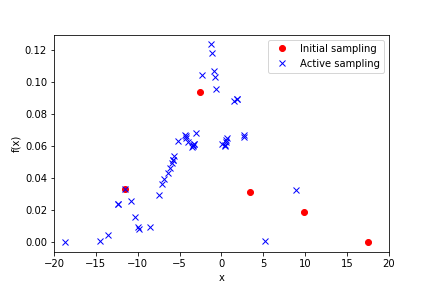
\includegraphics[width=0.35\linewidth]
		{figs/explopattern1g_aq_uncertainty_sampling.png}}
	
	\subfloat[PROP, moments.]{\label{fig11a}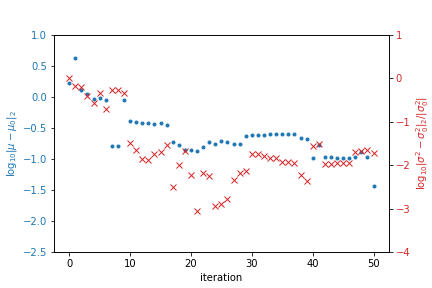
\includegraphics[width=0.35\linewidth]
	{figs/dmcil1g_aq_prospective.png}}
\subfloat[PROP, final result.]{\label{fig11b}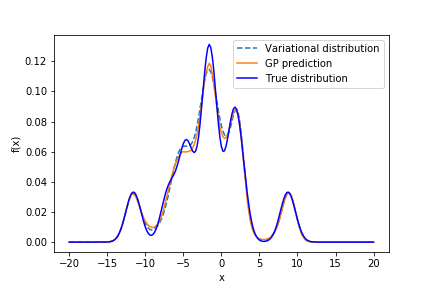
\includegraphics[width=0.35\linewidth]
	{figs/convgraphil1g_aq_prospective.png}}
\subfloat[PROP, sampling.]{\label{fig11b}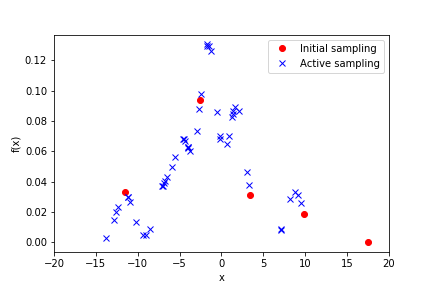
\includegraphics[width=0.35\linewidth]
	{figs/explopattern1g_aq_prospective.png}}
	
	\subfloat[MMLT, moments.]{\label{fig11a}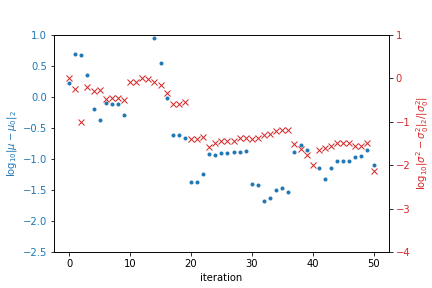
\includegraphics[width=0.35\linewidth]
	{figs/dmcil1g_aq_mmlt.png}}
\subfloat[MMLT, final result.]{\label{fig11b}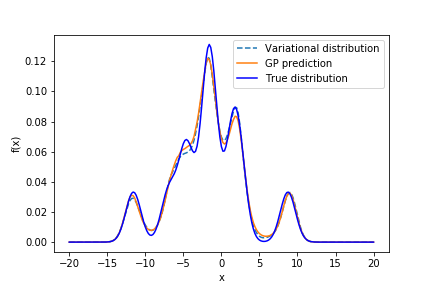
\includegraphics[width=0.35\linewidth]
	{figs/convgraphil1g_aq_mmlt.png}}
\subfloat[MMLT, sampling.]{\label{fig11b}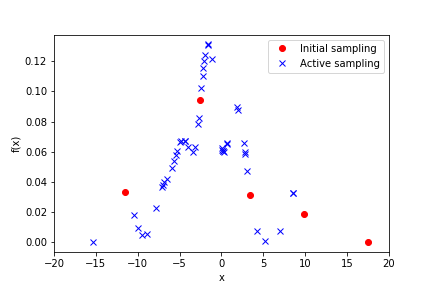
\includegraphics[width=0.35\linewidth]
	{figs/explopattern1g_aq_mmlt.png}}

	\subfloat[MMLT$_P$, moments.]{\label{fig11a}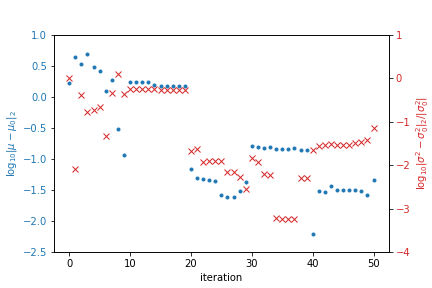
\includegraphics[width=0.35\linewidth]
	{figs/dmcil1g_aq_mmlt_prospective.png}}
\subfloat[MMLT$_P$, final result.]{\label{fig11b}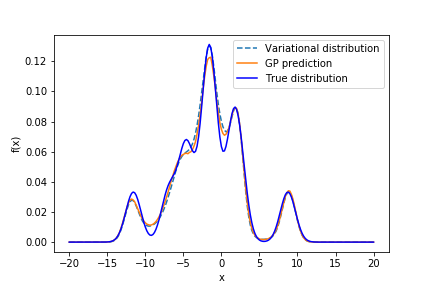
\includegraphics[width=0.35\linewidth]
	{figs/convgraphil1g_aq_mmlt_prospective.png}}
\subfloat[MMLT$_P$, sampling.]{\label{fig11b}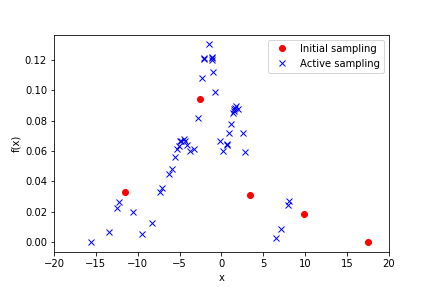
\includegraphics[width=0.35\linewidth]
	{figs/explopattern1g_aq_mmlt_prospective.png}}
	
	\caption[Accuracy analysis for different acquisition function.]{\label{acquisition} Convergence analysis for different acquisition function. Each row corresponds to acquisitions US, PROP, MMLT and MMLT$_P$, respectively. The first column shows the accuracy of mean and covariance, the second column show the difference between the predicted density, the true density and the GP approximation of the density, and the third column shows the places where the function was evaluated.}
\end{figure}

\newpage
\section{N-d toy examples}
In this section, we consider the algorithm performance on a set of toy examples, the same ones considered in \cite{Acerbi_2018}. Code for this section can be found in \url{https://github.com/DFNaiff/Dissertation/tree/master/tests_dissertation/toy}.

Three classes of test cases were considered:
\begin{itemize}
\item \textit{Lumpy}, a mixture of multivariate Gaussians
\begin{equation}
f(x) = \sum_{i=1}^{12} w_i \mathcal{N}(x;\mu_i,\Sigma_i),
\end{equation}
with $(w_1,\ldots,w_{12}) \sim \text{Dir}(1,\ldots,1)$, $\mu_i \sim \text{Unif}([0,1]^D)$ and $\Sigma = \text{diag}(\sigma_1^2,\ldots,\sigma_n^2)$, with $\sigma_i^2 \sim \text{Unif}(0.2,0.6)$. This distribution tests the algorithm performance in presence of possible multimodalities.

\item \textit{Cigar}, a anisotropic Gaussian distribution
\begin{equation}
f(x) = \mathcal{N}(x;0,\Sigma),
\end{equation}
where $\Sigma = Q \Lambda Q^T$, with $\Lambda = (10.0,0.1,\ldots,0.1)$, and $Q$ sampled from the uniform measure in the special orthogonal group. This distribution tests the algorithm performance in presence of large anisotropy.

\item \textit{Student-t}, a product of t distributions 
\begin{equation}
f(x) =  \prod_{d=1}^D \mathcal{T}(x_i;\nu_i),
\end{equation}
with $\nu_i \sim \text{Unif}(2.5,2+0.5D)$. This distribution tests the algorithm performance in presence of heavy tails \footnote{For both \textit{Cigar} and \textit{Student-t}, BVBMC was applied to an unnormalized density.} \footnote{Originally, $\nu_i = 2.5$ for every $i$, which assured reasonably heavy tails at every dimension. However, for comparison with \cite{Acerbi_2018}, this later case is not shown here}.
\end{itemize}

For each case, dimensions $D = 2,6,10$ where tested, and the BVBMC algorithm was run for $100$ iterations, with $10D$ initial samples. The GP kernel used were $k_{\text{PMat},\nu=2.5}$, with active evaluation at each iteration, according to an acquisition function randomly chosen between the pair $(\alpha_\text{PROP},\alpha_\text{MMLT})$. Every 20 steps, joint parameter updating was done, and pruning was done at each iteration, with $\beta = 10^{-3}$.

The algorithm performance was compared by checking the divergence between the true mean $\mu_0$ and the estimated mean $\mu$, in $\log_{10}||\mu - \mu_0||_2$, and between the true covariance $\Sigma_0$ and estimated covariance $\Sigma$, in $\log_{10}||\Sigma - \Sigma_0||_F/||\Sigma_0||_F$, where $||\cdot||_F$ denotes the Frobenius norm. The results are shown in Figure \ref{ndtoy}. For comparison with results given by the VBMC algorithm, shown in \cite{Acerbi_2018}, the "Gaussianized" symmetric KL divergence (gsKL) between the true distribution and estimated distribution is computed, which is defined as the symmetric KL divergence between two multivariate distributions with mean and covariance equals to the true distribution and the estimated distribution, respectively \footnote{In \cite{Acerbi_2018}, what is done are 15 evaluations for each case, and the median is taken. A better approach here would be doing the same thing for BVBMC, however due to time constraints this couldn't be done.}. The results are shown in Table \ref{toytable}. There it can be seen that, in general performance between BVBMC and VBMC was comparable, excluding the experiment with the \textit{Cigar} distribution with $D=10$, in which VBMC performed much better, and $D=2$, in which BVBMC performed better. \footnote{It should be noted that the BVBMC algorithm have used fewer evaluations, namely $120$,$160$ and $200$ for $D=2,6,10$, respectively, than the VBMC algorithm, which used $200$,$400$,$600$, for $D=2,6,10$. In this toy example this doesn't make a large computational difference, however in applications where likelihood evaluation is expensive it does.}

\begin{table}[]
	\begin{tabular}{l|l|l|l|l|l|l|}
		\cline{2-7}
		& \multicolumn{2}{l|}{Lumpy} & \multicolumn{2}{l|}{Cigar} & \multicolumn{2}{l|}{Student-t} \\ \cline{2-7} 
		& BVBMC         & VBMC        & BVBMC         & VBMC        & BVBMC         & VBMC        \\ \hline
		\multicolumn{1}{|l|}{D=2}  & $3.12 \times 10^{-3}$        & $6.5 \times 10^{-4}$         & $8.12 \times 10^{-3}$           & $2.1 \times 10^{-1}$         & $2.9 \times 10^{-1}$          & $2.0 \times 10^{-3}$         \\ \hline
		\multicolumn{1}{|l|}{D=6}  & $6.59 \times 10^{-2}$         & $ 3.5 \times 10^{-2}$         & $5.56 \times 10^{-1}$           & $ 1.07 \times 10^{-1}$        & $1.14 \times 10^{-1}$           & $2.3 \times 10^{-1}$         \\ \hline
		\multicolumn{1}{|l|}{D=10} & $1.19 \times 10^{-1}$           & $ 4.2 \times 10^{-1}$         & $1.29 $           &  $ 1.0 \times 10^{-1}$        & $2.56 \times 10^{-1}$           & $ 2.7 \times 10^{-1}$        \\ \hline
	\end{tabular}
	\caption{gsKL divergence between true distribution and estimated distribution. The values for VBMC were taken from the graphs in \cite{Acerbi_2018}.}\label{toytable}
\end{table}

\begin{figure}
	\centering
	\subfloat[Lumpy, means accuracy.]{\label{fig11a}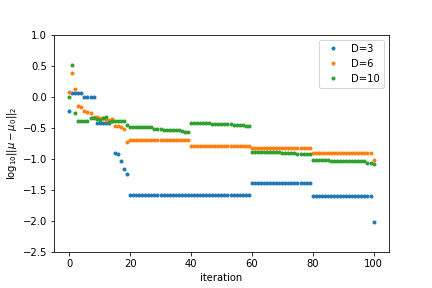
\includegraphics[width=0.5\linewidth]
		{figs/ex1b_mean.png}}
	\subfloat[Lumpy, covariances accuracy.]{\label{fig11b}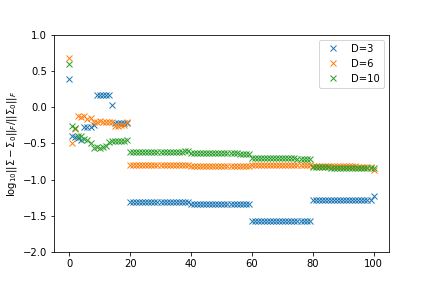
\includegraphics[width=0.5\linewidth]
		{figs/ex1b_cov.png}}

	
	\subfloat[Cigar, means accuracy.]{\label{fig11a}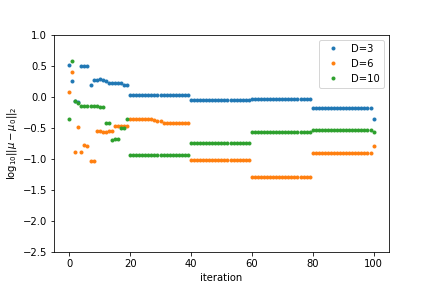
\includegraphics[width=0.5\linewidth]
		{figs/ex4b_mean.png}}
	\subfloat[Cigar, covariances accuracy.]{\label{fig11b}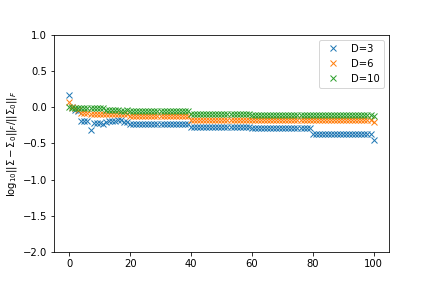
\includegraphics[width=0.5\linewidth]
		{figs/ex4b_cov.png}}

	\subfloat[Student-t, means accuracy.]{\label{fig11a}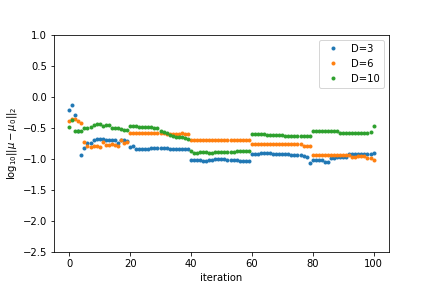
\includegraphics[width=0.5\linewidth]
	{figs/ex5b_mean.png}}
\subfloat[Student-t, covariances accuracy.]{\label{fig11b}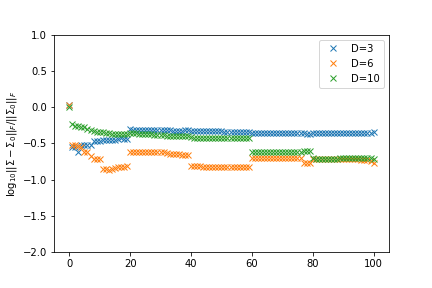
\includegraphics[width=0.5\linewidth]
	{figs/ex5b_cov.png}}

	
	\caption[Accuracy analysis for different N-d examples.]{\label{ndtoy} Accuracy analysis for different N-d examples. Each row corresponding to \textit{Lumpy}, \textit{Cigar} and \textit{Student-t}, respectively. The first column shows the accuracy of means, while the second column shows the accuracy of covariances.}
\end{figure}

\section{Contamination source estimation}
In this example, a contamination source location problem was considered, inspired by a problem in \cite{Bilionis_2013}. This problem is a toy example of an actual inverse problem, that is, given some sensor measurements of a contaminated field (the contamination may be, for instance, radiation), find where the contaminant as located, as well as its nature. Code for this section can be found in \url{https://github.com/DFNaiff/Dissertation/tree/master/tests_dissertation/source1d}.

The example consider a one-dimensional domain $B = [0,1]$, in which a contamination source $q(x,t)$ is inserted from $t=0$ to $t=t_s$. This source is modeled as
\begin{equation}
q(x,t) = q_0 \exp \left(-\frac{(x-x_0)^2}{2 \rho^2} \right) \mathbf{1}_{[0,t_s)}(t).
\end{equation}
The contaminant itself is assumed to follow the diffusion equation 
\begin{equation}
\frac{\partial}{\partial t} u(x,t) = \frac{\partial^2}{\partial x^2} u(x,t) + q(x,t), \quad x \in \text{int} B.
\end{equation}
Moreover, the initial contamination is considered to be $0$, while the walls are considered insulated, resulting in the boundary and initial value conditions
\begin{equation}
u(x,0) = 0, \; \frac{\partial}{\partial x} u(0,t) = \frac{\partial}{\partial x} u(1,t) = 0.
\end{equation}
It must be noticed that, for general domain length $L$ and diffusion coefficient $k$, using adimensionalization one can reduce the general problem to the above.

In this setting, at each wall $x=0,1$, four measurements of $u$ are made, for $t_m \in T_m = \{0.075,0.15,0.225,0.3,0.4\}$, resulting in the data 
\begin{displaymath}
 \mathcal{D} = \{\hat{u}(x_m,t_m)\}_{x_m \in \{0,1\},t_m \in T_m}.
\end{displaymath}
Moreover, the measurements are assumed to be noisy, with $\hat{u}(x_m,t_m) = u(x_m,t_m) + \epsilon$, $\epsilon \sim \mathcal{N}(0,\sigma^2)$. The noise parameter $\sigma^2$ is assumed to follow a prior $\text{InvGamma}(\alpha,\beta)$. This allows us to marginalize out $\sigma^2$, letting $\hat{u}(x_m,t_m)$ be distributed according to the generalized t-distribution \footnote{If $T_0$ follows a (standardized) t-distribution, with $nu$ degrees of freedom, then $T = \sigma T_0 + \mu$ follows a generalized t-distribution denoted by $\mathcal{T}(\mu,\sigma^2,\nu)$} with $2\alpha$ degrees of freedom $\mathcal{T}(u(x_m,t_m),\beta/\alpha,2 \alpha)$. 

The setting above results in a 4-dimensional inference problem, for the variables $(x_0,t_s,q_0,\rho)$, with likelihood
\begin{equation}
 p(\mathcal{D}|x_0,t_s,q_0,\rho) = \prod_{x_m \in \{0,1\},t_m \in T_M} \mathcal{T}(\hat{u}(x_m,t_m);u(x_m,t_m),\beta/\alpha,2 \alpha).
\end{equation}
Given priors for $x_0$,$t_s$,$q_0$ and $\rho$, the associated posterior distribution for the parameters becomes 
\begin{equation}\label{posteriorsource}
p(x_0,q_0,t_s,\rho|\mathcal{D}) \propto p(\mathcal{D}|x_0,q_0,T_s,\rho) p(x_0)p(q_0)p(\rho)p(t_s).
\end{equation}

A synthetic data $\mathcal{D}$ was generated, with the parameters given in Table \ref{sourcetable}, first row. The measurement noise was $\sigma^2 = 10^{-2}$, and the equation was simulated using a finite differences routine. The priors for the values to be inferred were set as \footnote{The Half-Cauchy distribution was used here as to represent a non-informative prior.}
\begin{equation}
\begin{split}
& p(x_0) = \text{Unif}(x_0;0,1) \\ 
& p(t_s) = \text{Unif}(t_s;0,0.4) \\
& p(q_0) = \text{HalfCauchy}(q_0;10) \\ 
& p(\rho) = \text{HalfCauchy}(\rho;0.1)
\end{split}
\end{equation}
In \eqref{posteriorsource}, $u(x,t)$ is also calculated by finite differences.

\begin{table}[h]
	\centering
	\begin{tabular}{l|l|l|l|l|}
		\cline{2-5}
		& $x_0$ & $t_s$ & $q_0$  & $\rho$ \\ \hline
		\multicolumn{1}{|l|}{True}  & 0.230 & 0.300 & 6.366  & 0.050  \\ \hline
		\multicolumn{1}{|l|}{BVBMC mean} & 0.328 & 0.213 & 5.435  & 0.140  \\ \hline
		\multicolumn{1}{|l|}{EMCEE mean} & 0.352 & 0.206 & 10.228 & 0.218  \\ \hline
		\multicolumn{1}{|l|}{BVBMC HDP 70\%} & $(1.1 \cdot 10^{-4},0.43)$ & $(0.12, 0.36)$ & $(1.0, 6.7)$ & $(2.7 \cdot 10^{-3}, 0.1)$  \\ \hline
		\multicolumn{1}{|l|}{EMCEE HDP 70\%} & $(3.4 \cdot 10^{-4}, 0.45)$ & $(0.08, 0.33)$ & $(0.4,10.3)$ & $(2.1 \cdot 10^{-3}, 0.1)$  \\ \hline
	\end{tabular}
	\caption{\label{sourcetable} Comparison of the true parameter of the problem (first row), the estimated means using BVBMC (second row) and EMCEE (third row), and 70\% highest posterior density interval for BVBMC and EMCEE.}
\end{table}

The BVBMC algorithm assumes that the distribution to be estimated has support in $\mathbb{R}^D$. This is not the case for the problem above, since $x_0$ and $t_s$ have both bounded support, while $q_0$ and $\rho$ have positive support. In order to apply the BVBMC algorithm, inference was made on the warped variables $\tilde{x}_0,\tilde{t}_s,\tilde{q}_0,\tilde{\rho}$, all of them with support in $\mathbb{R}$, such that  \footnote{The 0.4 factor here is due to the fact that $t_s$ lies between 0 and 0.4.}:
\begin{equation}
\begin{split}
 & x_0 = \text{sigmoid}(\tilde{x}_0) \\
 & t_s = 0.4 \times \text{sigmoid}(\tilde{t}_s)  \\
 & q_0 = \exp(\tilde{q}_0) \\
 & \rho = \exp(\tilde{\rho}), \\
\end{split}
\end{equation}
with
\begin{equation}
\text{sigmoid}(x) = \frac{1}{1+e^{-x}}.
\end{equation}
This results in the posterior distribution for the warped variables
\begin{equation}
 p(\tilde{x}_0,\tilde{t}_s,\tilde{q}_0,\tilde{\rho}|\mathcal{D}) \propto p(x_0,q_0,t_s,\rho|\mathcal{D}) \text{sigmoid}'(\tilde{x}_0) \text{sigmoid}'(\tilde{t}_s) \exp(\tilde{q}_0) \exp(\tilde{\rho})
\end{equation}

The BVBMC algorithm was applied to the problem, with the following setup:
\begin{itemize}
	\item The kernel used was $k_{\text{PMat},3/2}$ (both $k_{\text{PMat},5/2}$ and $k_{\text{SQE}}$ were also tested, with mixed results).
	\item The algorithm was initialized with 40 samples from the prior. After this, before the training loop, 40 more evaluations points were chosen by using the $\alpha_{MMLT}$ acquisition function.
	\item The algorithm was then run for 100 iterations, with an evaluation point chosen at each iteration, with the acquisition function chosen randomly between $\alpha_\text{{MMLT}}$ and $\alpha_\text{{PROP}}$. At each 20 iterations, the parameters were jointly optimized.
\end{itemize}

The predicted mean is shown in Table \ref{sourcetable}, second row. It can be seen that the estimated source location was relatively accurate, compared to the original one, while estimates for $\rho$ and $q_0$ where reasonable, and the estimate for $t_s$ did not deviate far from the prior mean. The resulting marginal univariate and bivariate distributions are shown in Figure \ref{sourcevbhistogram}.

\begin{figure}
	\centering
	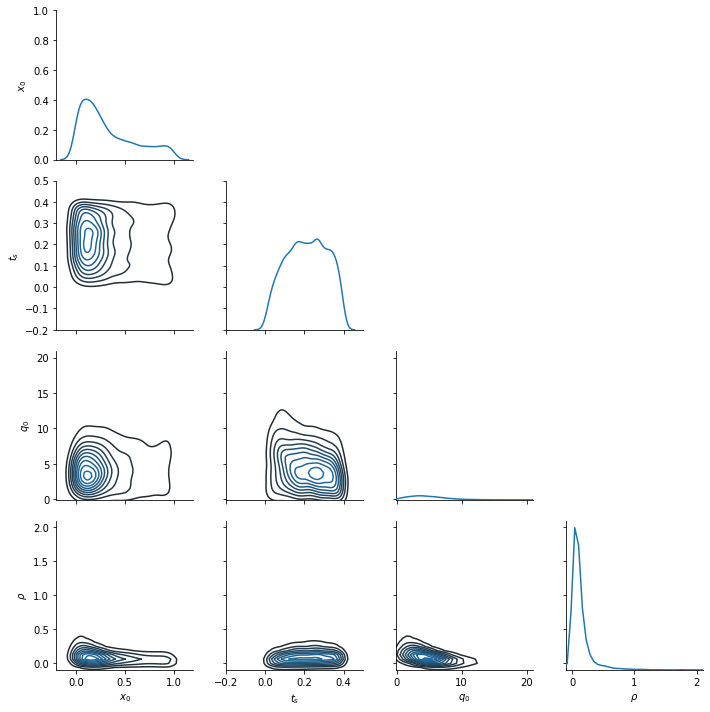
\includegraphics[width=0.8\linewidth]{figs/sourceproblemhistogramsvb.png}
	\caption[KDE plots of estimated marginals with BVBMC. On diagonal.]{KDE plots of estimated marginals with BVBMC. On diagonal, marginal univariate distributions for $x_0$,$t_s$,$q_0$ and $\rho$ are shown, while off-diagonal, the corresponding bivariate marginals for each pair is shown.}
	\label{sourcevbhistogram} 
\end{figure}

For comparison, the EMCEE algorithm \cite{Foreman_Mackey_2013}, which is a MCMC algorithm usually used for problems in astrophysics, was also tested. The EMCEE ran with $10$ walkers and $10000$ steps for each walker, using burn-in in the first $1000$ steps. The resulting estimated means is shown in Table \ref{sourcetable}, third row. It can be seem that in general the estimates were in the BVBMC algorithm, except for $q_0$, in which BVBMC seems to be more precise. The resulting marginal univariate and bivariate distributions are shown in Figure \ref{sourcevbhistogram}, showing some resemblance with the results found in BVBMC.

\begin{figure}
	\centering
	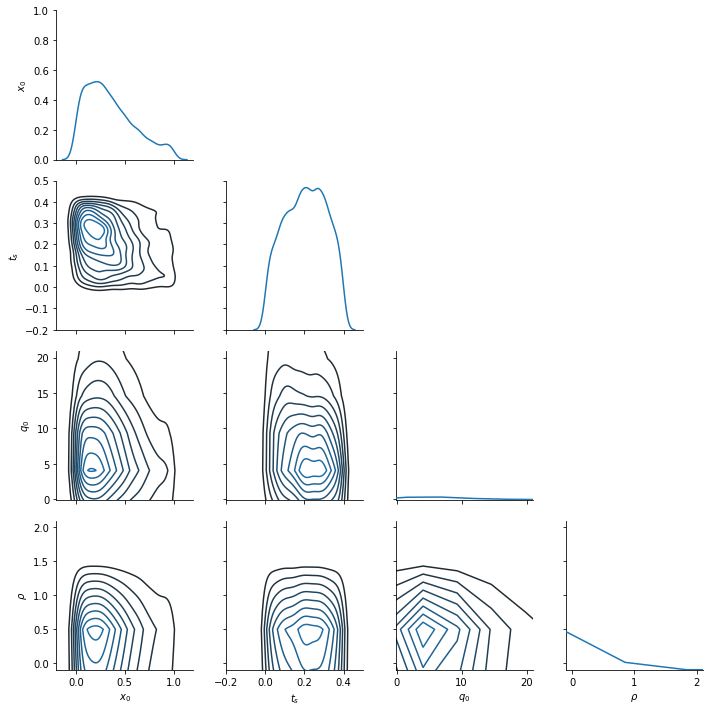
\includegraphics[width=0.8\linewidth]{figs/sourceproblemhistogramsemcee.png}
	\caption[KDE plots of estimated marginals with EMCEE. On diagonal.]{KDE plots of estimated marginals with EMCEE. On diagonal, marginal univariate distributions for $x_0$,$t_s$,$q_0$ and $\rho$ are shown, while off-diagonal, the corresponding bivariate marginals for each pair is shown.}
	\label{sourceemceehistogram} 
\end{figure}

\section{Checking performance}
In practice, one does not know the true posterior for doing comparison, and there must be some way to check whether BVBMC arrived at a good posterior.

Two sources of error may arise in the BVBMC estimate and the true posterior: Whether the variational proposal does not approximate well the GP surrogate model, or the GP surrogate model does not approximate well the true  unnormalized posterior. The first case may be checked using some rough estimate of the KL divergence between the variational proposal and the surrogate model, and is implemented in the method \textit{kl\_vb\_bmc} of the associated package. 

Checking whether the GP surrogate model resembles the true model may be harder. One option is to use leave-one-out testing \cite{Rasmussen06}, but one must consider that one does not care about accuracy in places where the unnormalized posterior does not contribute in probability mass. A heuristic to address this problem was not developed by the author.



